% Здесь пишется содержание первой главы
%
\chapter{\MakeUppercase{Разведочный анализ данных с использованием PySpark}}\label{ch:first}
\section{Постановка задачи разведочного анализа}\vspace{\baselineskip}

Разведочный анализ датасета - это первый этап в процессе анализа данных, который состоит из нескольких шагов. Цель этого этапа - получить общее представление о данных и их характеристиках, чтобы понять, какие методы анализа могут быть применены.

Основные цели разведочного анализа датасета включают:
\begin{enumerate}
\item Определение структуры данных: Разведочный анализ помогает определить, как выглядит ваш датасет – сколько столбцов (признаков) и строк (данных), какие типы данных используются (числовые, категориальные и т.д.).
\item Понимание распределения данных: Этот этап включает в себя проверку на наличие отсутствующих значений, выбросов или аномалий в данных.
\item Изучение основных характеристик данных: Определение среднего значения, моды, медианы и стандартного отклонения для числовых признаков; подсчет количества уникальных категорий для категориальных признаков.
\item Выявление взаимосвязей между переменными: Этот этап помогает понять, какие признаки могут влиять на другие в вашем датасете.
\item Визуализация данных: Построение графиков и диаграмм для наглядного представления данных и их распределения.
\end{enumerate}
Все эти шаги важны для того, чтобы понять ваши данные и выбрать правильные методы для дальнейшего анализа или машинного обучения.


\vspace{\baselineskip}\section{Описание датасета}\vspace{\baselineskip}

%Здесь требуется описать выбранный датасет, привести ссылку на него, охарактеризовать его тематику, объем, количество признаков. Вкратце нужно описать признаки датасета (допускается описывать не все признаки, а только те, которые используются в исследовании).
%Также, можно сослаться на источники, например, в \cite{karau2015spark, koirala2020pyspark, white2013hadoop, Tekdogan2022} рассматривается материал об ... Часть информации можно оформить в виде таблицы, но избегайте слишком длинных таблиц. На каждую таблицу должна быть ссылка в тексте, как, например, на таблицу \ref{tab:features}, в которой приведен пример описания признаков.

В приведенном датасете рассматриваются квартиры и их атрибуты для расчёта платы, такие как: площадь квартиры, её тип, использованное количество энергии, расход горячей воды и т.д. Таким образом из всех имеющихся признаков определяется рейтинг квартиры. Сам датасет весит более 20 Гб, но для работы с ним нам пришлось его обрезать до 5 Гб \cite{https://www.kaggle.com/datasets/tyagia1/epcratingsenglandjuly203}. Выбраны определенные 10 столбцов признаков для выполнения разведочного анализа.

\begin{table}[]
    \centering
    \begin{tabularx}{\textwidth}{|X|X|}
        \hline
        \multicolumn{1}{|c|}{Признак}  & \multicolumn{1}{c|}{Расшифровка признака}   \\ \hhline{|=|=|}
        LMK\_KEY					& Первичный ключ      \\ \hline
        ADDRESS					& Адрес                       \\ \hline
        CURRENT\_ENERGY\_EFFICIENCY	&  Эффективность энергии      \\ \hline
        PROPERTY\_TYPE                             	& Тип квартиры                       \\ \hline
        INSPECTION\_DATE                          	& Дата инспекции      \\ \hline
        HEATING\_COST\_CURRENT             	& Затраты на обогрев                       \\ \hline
        HOT\_WATER\_COST\_CURRENT	& Затраты на горячую воду      \\ \hline
        TOTAL\_FLOOR\_AREA                       	& Площадь                       \\ \hline
        NUMBER\_HABITABLE\_ROOMS       	& Количество обитаемых комнат     \\ \hline
        NUMBER\_HEATED\_ROOMS          	& Количество комнат с подогревом                       \\ \hline
    \end{tabularx}
    \caption{Таблица признаков}
    \label{tab:features}
\end{table}

\vspace{\baselineskip}\section{Определение пропущенных значений}\vspace{\baselineskip}

%Обратите внимание, что приведенная здесь структура раздела не является жестким требованием, а служит примером оформления. При необходимости, её можно корректировать в разумных пределах.
%При необходимости можно вставить рисунок и сослаться на него: на рисунке \ref{fig:HadoopEcoSystem} приведена иллюстрация экосистемы Hadoop. Обратите внимание, что таблицы и рисунки являются <<плавающими>> объектами: они могут располагаться не в месте их непосредственного объявления, а в некоторой близости от него.
%\begin{figure}
 %   \centering
 %   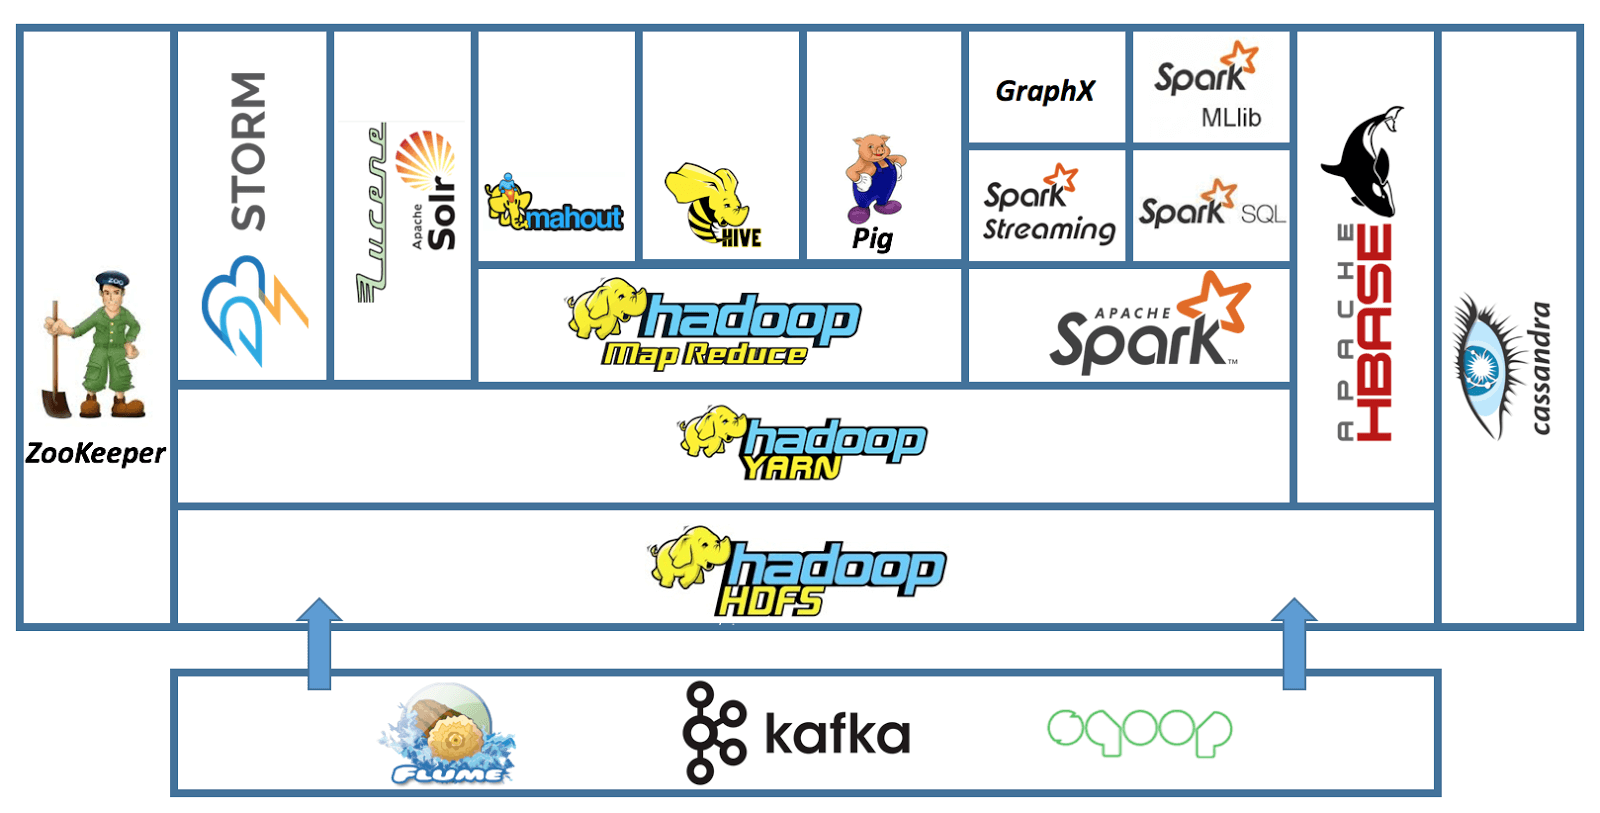
\includegraphics[width=\textwidth]{Content/Images/HadoopEcoSystem.png}
%    \caption{Иллюстрация экосистемы Hadoop}
%    \label{fig:HadoopEcoSystem}
%\end{figure}

%Также, вот пример списка:
При анализе мы предполагали, где  могут встречаться пропущеннные значения. С помощью команды count\_nulls мы определяли количества пропущенных значений в том или ином столбце. Ниже приведен список признаков, где пропущенные значения были недопустимы

А здесь -- аналогичный нумерованный список:

\begin{enumerate}
    \item ADDRESS3;
    \item HEATING\_COST\_CURRENT;
    \item NUMBER\_HABITABLE\_ROOMS
    \item NUMBER\_HEATED\_ROOMS
\end{enumerate}
\par После определения количества пропущенных значений мы работали с этими критериями мы их обрабатывали разными способами.
\par У ADDRESS3 более 90\% значений пропущены, этот столбец был удален в целях упрощения работы с датасетом.
\begin{code}
df = df.drop("ADDRESS3")
df.show()
\end{code}
В аналогичном случае можно было бы заменить пропущенные значения на значение Unknown
\begin{code}
df = df.fillna({"PROPERTY\_TYPE": "Unknown"})
count\_nulls(data=df, column\_name="PROPERTY\_TYPE")
\end{code}

\par В столбце HEATING\_COST\_CURRENT было пропущенно значений меньше половины, значит, можно попытаться обработать эти данные. Была создана функция позволяющая рассчитывать статистические показатели данных в столбцах и строить диаграмму "ящик с усами" для оценки наличия выбросов: "plot\_boxplots".
\begin{figure}
    \centering
    \includegraphics[width=\textwidth]{Content/Images/vibroses.png}
    \caption{Выбросы в HEATING\_COST\_CURRENT}
    \label{fig:VHCC}
\end{figure}
В результате получился boxplot с сильными выбросами в нескольких точках. Удалим строки, их содержащие, и убедимся, что потеряна небольшая часть данных и заменим пропуски средним значением признака.
\begin{code}
df.filter(col("HEATING\_COST\_CURRENT") > 8000).count()
df = df.filter(col("HEATING\_COST\_CURRENT") < 8000)
mean\_cost = df.select(mean(col("HEATING\_COST\_CURRENT"))).collect()[0][0]
mean\_cost
df = df.fillna({"HEATING\_COST\_CURRENT": mean\_cost})
\end{code}

\par В столбцах NUMBER\_HABITABLE\_ROOMS и NUMBER\_HEATED\_ROOMS содержатся пропущенные значения с типом float, заменим их на значения 0.0

\begin{code}
df = df.fillna({"NUMBER\_HABITABLE\_ROOMS": 0.0})
df = df.fillna({"NUMBER\_HEATED\_ROOMS": 0.0})
\end{code}

%%А вот формула, которая связывает между собой синус, косинус и тангенс.

%\begin{equation}
%    \label{eq:formula}
%    \tg \alpha = \frac{\sin \alpha}{\cos \alpha}.
%\end{equation}

%Ну, и ссылка на неё: формула (\ref{eq:formula}) выражает связь тригонометрических функций.

\vspace{\baselineskip}\section{Расчет корреляции между количественными признаками}\vspace{\baselineskip}

Рассчет корреляции между количественными признаками — это процесс, который позволяет определить степень и направление взаимосвязи между двумя или более переменными. Корреляция отражает насколько часто значения одной переменной изменяются вместе с изменениями в другой переменной.


Существует два основных типа корреляции:

\begin{enumerate}
\item Позитивная корреляция: Это ситуация, когда значения двух переменных меняются в одно и то же направление. Например, если при увеличении одной переменной (например, времени) увеличивается и другая (например, расстояние), это будет показывать положительную корреляцию.
\item Негативная корреляция: Это ситуация, когда значения двух переменных меняются в противоположных направлениях. Например, если при увеличении одной переменной (например, времени) уменьшается другая (например, расстояние), это будет показывать негативную корреляцию.
\end{enumerate}

\par Рассчитать корреляцию между количественными признаками можно с помощью различных статистических методов. Наиболее распространенным из них является коэффициент корреляции Пирсона, который показывает степень и направление линейной связи между двумя переменными.

Коэффициент корреляции Пирсона (r) вычисляется по формуле:

$$r = \frac{\sum_{i=1}^{n}(x_i - \bar{x})(y_i - \bar{y})}{\sqrt{\sum_{i=1}^{n}(x_i - \bar{x})^2 \sum_{i=1}^{n}(y_i - \bar{y})^2}}$$


В большинстве случаев используется коэффициент корреляции Пирсона для измерения линейной связи между двумя количественными признаками. Коэффициент Пирсона, обозначенный как r, варьируется от -1 до 1:
\begin{enumerate}
\item Если r близок к 1, то связь между переменными очень сильная и положительная.
\item Если r близок к -1, то связь между переменными очень сильная и негативная.
\item Если r близок к 0, то между переменными нет линейной связи.
\end{enumerate}

Важно отметить, что корреляция не говорит о причине и последствии между двумя переменными; она просто показывает, насколько сильно значения одной переменной изменяются в зависимости от значений другой.

\par Корреляционные коэффициенты часто используются для анализа и визуализации данных, чтобы определить взаимосвязь между различными признаками. Они могут помочь в выборе переменных для моделей машинного обучения или в выявлении закономерностей в данных.

Код расчёта:
\begin{code}
def compute_and_visualize_correlation_matrix(data: DataFrame, 
                                             columns: list[str]) -> None:
    """
    Вычисляет и визуализирует корреляционную матрицу для указанных 
    колонок в DataFrame PySpark.

    Args:
        df (DataFrame): DataFrame PySpark.
        columns (list[str]): Список колонок для вычисления корреляции.

    Returns:
        None
    """
    # Вычисление корреляционной матрицы
    corr_matrix = {}
    for col1 in columns:
        corr_matrix[col1] = {}
        for col2 in columns:
            corr_value = data.select(corr(col1, col2)).collect()[0][0]
            corr_matrix[col1][col2] = corr_value

    # Преобразование корреляционной матрицы в DataFrame Pandas для визуализации
    corr_matrix_pd = pd.DataFrame(corr_matrix)

    # Построение и визуализация корреляционной матрицы
    plt.figure(figsize=(10, 8))
    sns.heatmap(corr_matrix_pd, annot=True, cmap='coolwarm', linewidths=0.5)
    plt.title('Correlation Matrix')
    plt.show()
\end{code}

%Здесь можно продемонстрировать пример включения фрагмента кода в текст работы. И заодно добавить еще пару ссылок \cite{spark2022official, zaharia2021lakehouse}.
%\begin{code}
%import matplotlib.pyplot as plt
%import numpy as np
%x = np.linspace(0, 10, 100)
%y = np.sin(x)
%plt.figure(figsize=(10, 6))
%plt.plot(x, y, label='sin(x)', color='blue', linewidth=2)
%plt.title('График функции sin(x)', fontsize=16)
%plt.xlabel('x', fontsize=14)
%plt.ylabel('sin(x)', fontsize=14)
%plt.legend()
%plt.grid(True)
%plt.show()    
%\end{code}

%Здесь продолжается текст. Не забывайте, что фрагмент кода не должен превышать половины страницы -- затем должен следовать текст.

\vspace{\baselineskip}\section{Выводы}\vspace{\baselineskip}

В результате полученной работы была разработана корреляционная матрица, демонстрирующая наличие корреляции между количественными признаками.

\begin{figure}
    \centering
    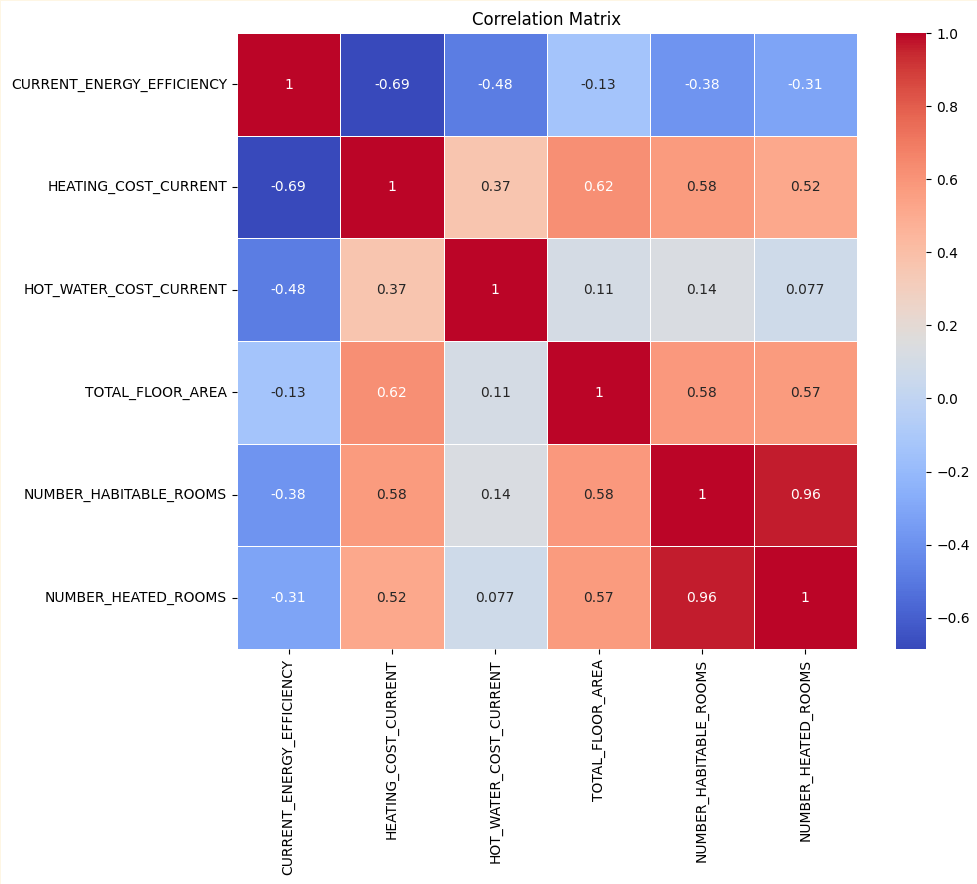
\includegraphics[width=\textwidth]{Content/Images/CorMatrixOfDataset.png}
    \caption{Корреляционная матрица датасета}
    \label{fig:CorMatrixOfDataset}
\end{figure}

Здесь наблюдается наибольшая зависимость  обитаемых и обогреваемых комнат от площади самой квартиры.
